\documentclass[a4paper, 11pt]{report}
\usepackage{epsfig}
\usepackage{graphics}
\usepackage{multirow}
\usepackage{multicol}
\usepackage{fancyhdr}
\usepackage{lastpage}
\usepackage{latexsym}
\usepackage[hang, scriptsize, bf]{caption}

\usepackage[utf8]{inputenc}

\usepackage{enumerate}

\usepackage{tikz}
\usepackage[european]{circuitikz}

\usepackage{stackengine}
\usepackage{scalerel}
\usepackage{xcolor}
\newcommand\dangersign[1][2ex]{%
  \renewcommand\stacktype{L}%
  \scaleto{\stackon[1.3pt]{\color{red}$\triangle$}{\tiny\bfseries !}}{#1}%
}
%-------------------------------------------------------------------------------

\textwidth      170mm
\textheight     240mm
\hoffset        -10mm 
\voffset        -10mm
\oddsidemargin   5mm
\evensidemargin -5mm
\topmargin	    -5mm

%-------------------------------------------------------------------------------

\newcommand{\eduTitle}{Zadání laboratoře}
\newcommand{\eduID}{6}
\newcommand{\eduTopic}{Operační zesilovač}
\newcommand{\eduDetails}{
\footnotesize
Cíl: 
Experimentálně ověřit chování a vybrané aplikace operačního zesilovače.
}
%
\newcommand{\subjIDlong}{Elektronika pro informační technologie}
\newcommand{\schoolDlong}{Vysoké učení technické v Brně}
\newcommand{\schoolDshort}{VUT v Brně}
\newcommand{\facultylDlong}{Fakulta informačních technologií}
\newcommand{\facultylDshort}{FIT}
%
\newcommand{\subjIDshort}{IEL}
%
\newcommand{\actYear}{2024}
\newcommand{\acadYear}{2024/2025}


\usepackage[hidelinks]{hyperref}

%-------------------------------------------------------------------------------

\newcommand*\circled[1]{\tikz[baseline=(char.base)]{
            \node[shape=circle,draw,inner sep=2pt] (char) {#1};}}

%-------------------------------------------------------------------------------

\newcounter{cntInfo}
\newcommand{\info}[3]{\refstepcounter{cntInfo}
\paragraph*{
\circled{\thecntInfo}~{\sc \fbox{#1}} {\sc #2}  
} 
\paragraph{\textmd{#3}} }


\renewcommand{\figurename}{Obrázek}
\renewcommand{\tablename}{Tabulka}


\newcommand\encircle[1]{%
  \tikz[baseline=(X.base)] 
    \node (X) [draw, shape=circle, fill=yellow, inner sep=0] {\strut #1};}

\newcommand\encircleII[1]{%
  \tikz[baseline=(X.base)] 
    \node (X) [draw, shape=circle, fill=none, inner sep=0] {\strut #1};}


%-------------------------------------------------------------------------------

\begin{document}

%-------------------------------------------------------------------------------

\pagestyle{fancy}
\renewcommand{\headrulewidth}{0pt}
\renewcommand{\theenumi}{\Alph{enumi}}  
\lhead{}
\chead{}
\rhead{}
\lfoot{\centering
\tiny \itshape \eduTitle ~č. \eduID \hspace{0.1mm} z předmětu \subjIDshort \hspace{1mm} 
(ak. r. \acadYear). \copyright~\actYear~Josef~Strnadel,~\facultylDshort~\schoolDshort. Připomínky zasílejte na \href{mailto:strnadel@fit.vut.cz}{strnadel@fit.vut.cz}\\ 
Časové razítko PDF dokumentu [\pdfcreationdate]. 
Sazba byla provedena systémem \LaTeX.
 }
\cfoot{}
%-------------------------------------------------------------------------------

\begin{center}
\scalebox{0.1}{
\includegraphics{FIT_cernobile_CZ.pdf}}
\parbox{120mm}{
\textsc{\footnotesize\schoolDlong}, 
\textsc{\footnotesize\facultylDlong}\\
}
{
\Large
\textsc{\subjIDlong} (\textsc{\subjIDshort}), \textsc{ak. r. \acadYear}}

\hrulefill

\vspace{4mm}
\parbox{\linewidth}{
\centering
%
{\Huge \textsc{\eduTitle~č.~\fbox{\eduID}}}\\
{\textsc{,,\eduTopic''}}\\

}

\end{center}

{\it \eduDetails}

\hrulefill

%-------------------------------------------------------------------------------
\vspace{-1mm}
\info{Motivace}{aneb ,,Proč tomu věnovat čas a jaké kompetence lze získat ?''\vspace{-3mm}}{
Na základě sady experimentů budete moci ověřit, pochopit a objasnit princip činnosti 
vybraných praktických zapojení\protect\footnote{napěťový komparátor, 
zesilovač či 
součtový zesilovač 
(viz Obr. \ref{fig:oz_apps})} založených na operačním zesilovači (OZ).
}

%-------------------------------------------------------------------------------
\info{Výstup a způsob jeho hodnocení}{aneb ,,Co se ode mne očekává a co za to ?''\vspace{-3mm}}{
Za konstrukci a experimentální ověření činnosti
napěťového komparátoru,
zesilovače
a
sumátoru
na bázi OZ
a 
za, experimentálně podložené, 
objasnění 
chování zkoumaných obvodových zapojení
a~nastínění jejich možného využití v praxi
lze získat až {\bf 3 body}.
}

%-------------------------------------------------------------------------------
\info{Prostředky}{aneb ,,Co je k dispozici ?''\vspace{-3mm}}{
~
}


\hspace{-8mm}
\parbox{15mm}{
\vspace{2mm}
\dangersign[8ex] 
}
\parbox{155mm}{
Zdroj ss. napětí s omezením proudu,
nepájivé pole, 
krabička s konstrukčními prvky (rezistory, OZ, vodiče), 
měřicí přístroje (multimetr, osciloskop).
\it
\\
\textcolor{red}{
Operační zesilovač (OZ) nevyjímejte z nepájivého pole! 
}
}
\\


%-------------------------------------------------------------------------------
\info{Základní schéma(ta)}{aneb ,,Z čeho se bude vycházet ?''\vspace{-3mm}}{
~
}




\ctikzset{amplifiers/fill=cyan!10, component text=center}
\ctikzset{resistors/fill=cyan!10, component text=center}

\begin{figure}[h]
\vspace{-4mm}
\centering
\parbox{50mm}{
\footnotesize
\centering
a) \hspace{2mm}
\scalebox{.225}{
\href{https://ww1.microchip.com/downloads/en/DeviceDoc/20001685E.pdf}{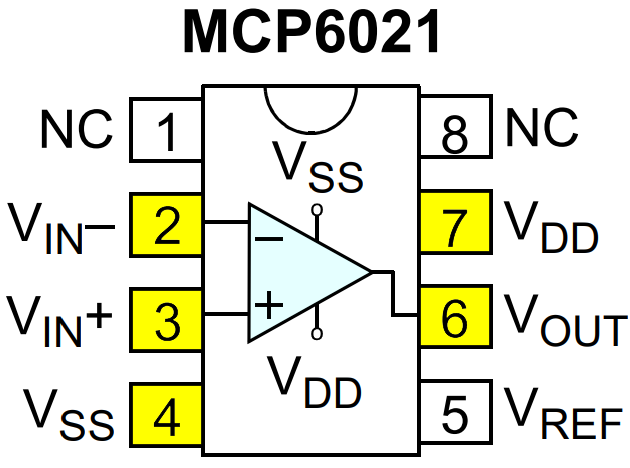
\includegraphics[trim=0 0mm 0 0mm, clip]{opamp-mcp6021.png}}
}
}
\hspace{16mm}
\parbox{40mm}{
\footnotesize
\centering
b) \scalebox{1.0}{
\begin{circuitikz}[]
\draw (0,0) 
node[op amp, 
noinv input down, anchor=+](OA){\texttt{OZ}} node[below] {\scalebox{1}{\encircle{3}}}
(OA.up) to [short, -o] ++(0,.5) node[below right] {\scalebox{1}{\encircle{4}}} node[above] {$V_{SS}$}
(OA.down) to [short, -o] ++(0,-.5) node[above right] {\scalebox{1}{\encircle{7}}} node[below] {$V_{DD}$}
(OA.-) node[above] {\scalebox{1}{\encircle{2}}}
(OA.out) node[above left] {\scalebox{1}{\encircle{6}}}
;
\end{circuitikz}
}
}

\vspace{-2mm}
\caption{
Pouzdro (a) a schematická značka (b) pro OZ typu \href{https://ww1.microchip.com/downloads/en/DeviceDoc/20001685E.pdf}{MCP6021};
význam vývodů je následující (NC představuje nezapojený/nevyužitý vývod): 
1 -- NC,
2 -- invertující vstup,
3 -- neinvertující vstup,
4 -- nižší potenciál zdroje napětí,
5~--~výstupní referenční napětí odpovídající $\frac{1}{2}(V_{DD}+V_{SS})$,
6 -- výstup,
7 -- vyšší potenciál zdroje napětí,
8 -- NC}
\label{fig:oz_schemas}
\end{figure}

{\bf Ideální OZ} má následující vlastnosti:
$\infty$ velké napěťové a proudové zesílení a vstupní odpor, nulový výstupní odpor, frekvenční nezávislost, nekonečně velké potlačení součtového signálu\footnote{signál společný oběma vstupům}. 
{\bf Reálný OZ} tyto vlastnosti nemá, ale přibližuje se jim\footnote{např. zesílením v řádu $10^5$ s maximem dosažitelným v zapojeních bez zpětné vazby; k základním parametrům OZ patří 
např. 
vstupní napěťová nesymetrie, 
potlačení vlivu změn napájecího napětí,
vstupní klidový proud a proudová nesymetrie,
vstupní rozdílová impedance,
maximální napájecí napětí,
potlačení souhlasného signálu, 
maximální dovolená výkonová ztráta
či
napěťové zesílení při otevřené smyčce bez zpětné vazby}.

\vspace{2mm}

\hspace{-8mm}
\parbox{15mm}{
\vspace{2mm}
\dangersign[8ex] 
}
\parbox{155mm}{
\it
Pozn.: 
Napětí $V_{OUT}$ je u reálného OZ
v rozmezí $V_{DD}$ až $V_{SS}$, tradičně $V_{DD}$ = $V_{CC}$, $V_{SS}$ = $-V_{CC}$.
$V_{OUT}$ většinou měříme oproti $(V_{DD}+V_{SS})/2$, 
tradičně oproti 0~V; jindy,
např. při $V_{DD} = V_{CC}$ a $V_{SS} = 0~V$,
však může být vhodnější měřit $V_{OUT}$ oproti $V_{CC}/2$ = $V_{REF}$. 
}


\newpage



%-------------------------------------------------------------------------------
\info{Postup samostatných činností}{aneb ,,Co dělat a na co si dát pozor ?''}{
~
}

\vspace{-9mm}

\begin{enumerate}[\bf {Experiment} 1:]

\item 
\begin{enumerate}[i)]

\item
{\bf Prostudujte} rozmístění vývodů OZ (Obr. \ref{fig:oz_schemas}a),
{\bf připojte} k OZ 
napájecí napětí\footnote{tj. 
$V_{SS} = 0~V$, 
$V_{DD} = 5~V$
}.

\item 
{\bf Zapojte} OZ 
dle Obr. \ref{fig:oz_apps}a --
jeden z uzlů \parbox{4mm}{\vspace{0mm}\scalebox{.75}{\encircle{A}}}, \parbox{4mm}{\vspace{0mm}\scalebox{.75}{\encircle{B}}} 
připojte na ss. napětí\footnote{tzv. referenční napětí (v rozmezí $V_{SS}$ až $V_{DD}$); nezaměňovat s $V_{REF}$ na vývodu \parbox{4mm}{\vspace{-1mm}\scalebox{.75}{\encircleII{5}}} OZ (viz Obr. \ref{fig:oz_schemas}a) !!!} ($V_{R}$),
druhý 
připojte na vhodný napěťový signál $v_{in}(t)$\footnote{signál
nad resp. pod úrovní $V_{R}$, popř.
procházející přes úroveň $V_{R}$}.
{\bf Sledujte}\footnote{oproti $V_{SS}$ či $V_{REF}$}
průběh
$v_{out}(t)$ 
a~{\bf zkoumejte}
závislost $v_{out}(t)$ na 
$v_{in}(t)$,
$V_{R}$\footnote{v případě zájmu činnosti zopakujte 
při prohozeném významu uzlů \parbox{4mm}{\vspace{0mm}\scalebox{.75}{\encircle{A}}}, \parbox{4mm}{\vspace{0mm}\scalebox{.75}{\encircle{B}}}}; {\bf předveďte} funkčnost vyučující(mu).

\end{enumerate}

\begin{figure}[h]
\vspace{-4mm}
\centering

\hspace{25mm}
\parbox{2mm}{
\vspace{-4mm}
\footnotesize
a)
}
\hspace{-32mm}
\scalebox{.9}{
\begin{circuitikz}[scale=0.8, transform shape]
\draw (0,0) 
node[above] {\encircle{A}} to[short, o-] ++(0.5,0)
to[R, l=$R_{+}$] ++(1.5,0)
node[op amp, noinv input up, anchor=+](OA){\texttt{OZ}}
(OA.-) to[R, l=$R_{-}$] ++(-1.5,0)
to[short, -o] ++(-.5,0) 
node[below] {\encircle{B}}
(OA.out) to[R, l=$R_{out}$] ++(1.5,0)
to[short, -o] ++(.5,0) node[below]{$v_{out}(t)$}
;
\node at(4.5,-1.85) {
\begin{math}
v_{out}(t) = 
  \left\{
    \begin{array}{ll}
      V_{DD} & V_A > V_B \\
      V_{SS} & V_A < V_B
    \end{array}
  \right.
\end{math}
}
;
\node at(0,-3.0) {}
;
\end{circuitikz}
}
%
\hspace{19mm}
%
\parbox{2mm}{
\vspace{-4mm}
\footnotesize
b)
}
\hspace{-27mm}
\scalebox{.9}{
\begin{circuitikz}[scale=0.8, transform shape]
\draw (0,0) 
node[below] {\encircle{A}} to[short, o-] ++(2.25,0)
node[op amp, noinv input up, anchor=+](OA){\texttt{OZ}}
(OA.-) 
  -- ++(0,-1) coordinate(FB) 
to[R, l=$R_1$] ++(-2,0) 
to[short, -o] ++(-.25,0)
node[below] {\encircle{B}}
(FB) to[R, l_=$R_2$, *-]  (FB -| OA.out) -- (OA.out)
to [short, *-o] ++(.5,0) node[above]{$v_{out}(t)$} node[below = 0mm] {\hspace{-6mm}\parbox{26mm}{\centering \vspace{2mm} =\\ $\pm  f(v_{in}(t), \frac{R_2}{R_1})$}}
;
\node at(0,-3.5) {}
;
\end{circuitikz}
}
%
\hspace{11mm}
%
\parbox{2mm}{
\vspace{-4mm}
\footnotesize
\hspace{-4mm}c)
}
\hspace{-20mm}
\scalebox{.9}{
\begin{circuitikz}[scale=0.8, transform shape]
\draw (0,0) coordinate(u0) 
node[left]{$x_ 0 = v_{in0}(t)$} to[short, o-] ++(0.5,0) 
to[R, l^=$R_0$] ++(2,0)
node[op amp, noinv input down, anchor=-](OA){\texttt{OZ}}
(OA.+) to[short, -o] ++(-.0, 0)
node[left=0.5mm]{\encircleII{5}}
node[left=8mm] {\parbox{8mm}{\centering $V_{REF}$}} 
(u0) ++(0,1)
node[left]{$x_1 = v_{in1}(t)$} to[short, o-] ++(0.5,0) coordinate(u1)
to[R, l^=$R_1$] ++(2,0) 
to[short, *-*] 
(OA.-)
(u0) ++(0,2)
node[left]{$x_2 = v_{in2}(t)$} to[short, o-] ++(0.5,0) coordinate(u2)
to[R, l^=$R_2$] ++(2,0) coordinate(u2B)
to[short, *-] 
(OA.-)
(OA.out)
to[short, *-] ++(0,2.5)
to[R, l_=$R_{FB}$] ++(-2,0)
to[short] (u2B)
(OA.out) 
to[short, -o] ++(.5,0) 
node[below] {$y = v_{out}(t)$ = }
node[below = 5mm] {\hspace{-4mm}= $-R_{FB}\cdot\sum_{k=0}^{2}\frac{x_k}{R_k}$}
;
;
\end{circuitikz}
\hspace{-4mm}
}

\vspace{-4mm}
\caption{Schémata k zapojení vybraných aplikací OZ: a) napěťový komparátor, b) napěťový zesilovač, c)~součtový zesilovač (sumátor) využitelný např. ke konstrukci číslicově-analogového převodníku (D/A, DAC)}
\label{fig:oz_apps}
\vspace{-0mm}
\end{figure}

\vspace{-2mm}
\item 
\begin{enumerate}[i)]
\item
V rámci zvolené studentské skupiny 
{\bf zapojte} OZ 
dle Obr. \ref{fig:oz_apps}b; jeden z uzlů \parbox{4mm}{\vspace{0mm}\scalebox{.75}{\encircle{A}}}, \parbox{4mm}{\vspace{0mm}\scalebox{.75}{\encircle{B}}} spojte s 
$V_{REF}$ (popř. $V_{SS}$)
a
na druhý 
přiveďte vhodný napěť. signál $v_{in}(t)$.
\item
{\bf Zkoumejte} 
vliv 
$R_1$, $R_2$ na 
$u_{out}(t)$; poté {\bf zvolte} 
$R_1$, $R_2$ tak, aby 
bylo dosaženo vyučujícím zadaného ne/invertujícího napěťového zesílení ($A_u = \frac{v_{out}(t)}{v_{in}(t)}$);
dosaže- ní $A_u$ {\bf ověřte} měřením; {\bf předveďte} funkčnost vyučující(mu). 

\end{enumerate}


\vspace{-1mm}
\item 
\begin{enumerate}[i)]
\item
V rámci zvolené studentské skupiny 
{\bf zapojte} OZ ve funkci 3bitového DAC
dle Obr. \ref{fig:oz_apps}c\footnote{trojici vstupních napětí 
chápejte jako vstupní 3bitovou informaci 
$x_2x_1x_0$ (kde 
$x_2$ 
je
nejvýznamnější,
$x_0$ nejméně významný bit;
vstupní log.0 chápejte jako $V_{REF}$, vstupní log.1 jako $V_{DD}$)
představující celé číslo z rozsahu 0--7};
hodnoty odporů 
$R_{FB}$,
$R_{2}$,
$R_{1}$,
$R_{0}$
{\bf zvolte} tak, aby 
vstup 
$x_2x_1x_0$
zajistil na výstupu OZ napětí (měřeno oproti $V_{REF}$) 
$y \approx - \frac{1}{4}\cdot hodnota(x_2x_1x_0)$.
\item
{\bf Odměřte} napětí $y$ pro dílčí vstupy, 
{\bf doplňte} chybějící údaje
v Tab.~\ref{tab1}\footnote{začněte doplněním chybějících ideálních hodnot -- získáte je výpočtem z příslušných vztahů (vzorců)},
vztah $y$ a $x_2x_1x_0$ {\bf znázorněte} grafem;
funkčnost zapojení {\bf předveďte} vyučující(mu).

\end{enumerate}




\vspace{-2mm}
\begin{table}[h]
\centering

\scalebox{0.7}{

\begin{tabular}{|c|c|c|c|c|c|c|c|c|c||c|c|c|c|c|c|}
\hline
\multicolumn{2}{|c|}{\hspace{0mm}\parbox{38mm}{\centering \vspace{2mm}$hodnota$($x_2x_1x_0$) [-]\vspace{2mm} $\rightarrow$}} 
& \parbox{8mm}{\centering 0} & \parbox{8mm}{\centering 1}& \parbox{8mm}{\centering 2}& \parbox{8mm}{\centering 3}& \parbox{8mm}{\centering 4}& \parbox{8mm}{\centering 5}& \parbox{8mm}{\centering 6}& \parbox{8mm}{\centering 7}
&
\multicolumn{2}{|c|}{Rezistor}  &
\parbox{8mm}{\centering $R_{FB}$}& \parbox{8mm}{\centering $R_{2}$}& \parbox{8mm}{\centering $R_1$}& \parbox{8mm}{\centering $R_0$}
\\
\hline
\hline
\parbox{12mm}{\vspace{4mm}\centering $\rightarrow$ napětí $y$ [V]\vspace{-6mm}} &\parbox{20mm}{\centering\vspace{0mm}ideální
\\(vypočtené)} &&&&&&&&
&
\multirow{2}{*}{\parbox{10mm}{\centering \vspace{2mm}odpor [$k\Omega$]}} &\parbox{18mm}{\centering \vspace{0mm}ideální\\(vypočtený)}&&&& 
\\
\cline{2-10}
\cline{12-16}
\parbox{12mm}{\vspace{10mm}}  & \parbox{30mm}{\centering\vspace{0mm}naměřené\\{(oproti $V_{REF}$)}} &&&&&&&&
&
&\parbox{28mm}{\centering \vspace{0mm}zvolený (dle odpor. řady Ex)}&&&& 
\\
\hline

\end{tabular}
}

\vspace{-3mm}
   \caption{Záznam hodnot k experimentu č. 3}
   \label{tab1}
   \vspace{-5mm}
\end{table}

\end{enumerate}


%-------------------------------------------------------------------------------
\vspace{-2mm}
\info{Shrnutí, vyhodnocení a interpretace výsledků}{aneb ,,Jaká jsou zjištění ?''\vspace{-4mm}}{
Napětí na výstupu OZ ($V_{OUT}$) je vždy v mezích napájecího napětí OZ. 
OZ dokáže 
vstupní signály vzájemně porovnávat, 
popř.
zesílit vstupní signál se zesílením $k \geq 1$ 
je-li signál přiváděn přes neinvertující ($+$) vstup
či
zesílit signál s $k \geq 0$, avšak také
změnit jeho fázi (znaménko), 
je-li přiváděn přes invertující ($-$) vstup.
V zapojení sumátoru má OZ schopnost sčítat vstupní signály.
\vspace{-1mm}
}

%-------------------------------------------------------------------------------
\vspace{-0mm}
\info{\vspace{-1mm}K zamyšlení/zapamatování}{aneb ,,Něco do dalšího studia a života.''\vspace{-4mm}}{
Řada aplikací OZ nebyla v této lab. zkoumána -- zmiňme např. využití OZ ke konstrukci derivátoru či integrátoru
pro
 řešení soustavy diferenciálních či integrálních rovnic pro počáteční podmínku určenou napětím na kondenzátoru.
V souvislosti s číslicovými zařízeními 
lze OZ využít 
např. 
v zapojení $n$bitového DAC
použitelného
k číslicově řízenému generování signálu o $2^n$ úrovních.
\vspace{-0mm}
}


\end{document}
